\chapter{Background and State-of-the-Art}
\label{chap.stateoftheart}
% This chapter, if desired, can be split into two chapters
% - Theoretical Background
% - Previous Results and Related Work

In the last decade we have seen a dramatic decrease in the cost of certain computation technologies and such phenomenon gave a birth of a new family of embedded control systems that are much better prepared for fluent, realistic interaction with the continuous physical world around them. For systems that combine physical world around us with the world of cybernetics, we use a term cyber-physical system. Although certain forms of CPS have been in industril use since 1980s, only recently has the technology for processors, wireless communication, and sensors matured to allow the production of components with impressive capabilities at a low cost \cite{Rajeev:PrinciplesCPS}.

Advance in the field of Cyber-physical systems will bring us closer to usage of high-speed, low-cost, and real-time embedded computers in technologies like electric networks that employ advanced monitoring \cite{Xue:SmartGrids}, networked autonomous vehicles \cite{Lee:DesignCPS} or prosthesis like neural controlled artificial leg \cite{Zhang:ArtificialLegs}. CPS are a research priority for both, government agencies (National Science foundation) and industry (automotive, avionics, medical devices).

\section{Cyber-Physical Systems}

The concept of a cyber-physical system is a generalization of embedded systems. An embedded system consists of hardware and software integrated within a mechanical or and electrical system designed for a specific purpose. As shown in Figure \ref{fig:CPS}, CPS consist of a computational unit, sensors, actuators and a physical world which it must observe and react on it. In a CPS the controller consists of discrete software concurrent components, operating in multiple modes of operation, interacting with the continuosly evolving physical environment. Examples of on-board sensors include a global positioning system (GPS) receiver, a camera or an infrared thermal sensor \cite{Rajeev:PrinciplesCPS}. CPS are reactive systems which interact with its environment in an ongoing manner. There is an endless loop of data collection and input evaluation throughout the time.

\begin{figure}
\centering
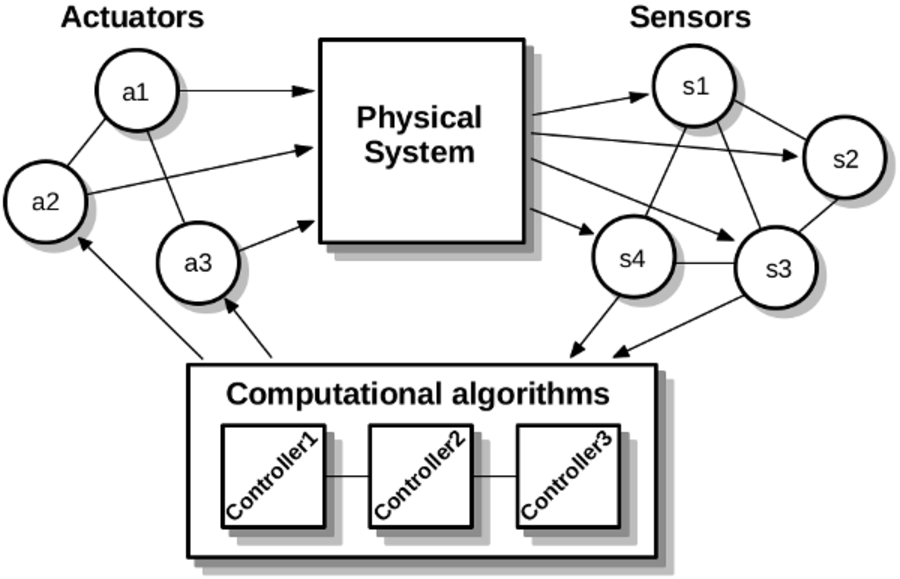
\includegraphics{pic/CPS_diagram_scaled}
\caption{Architecture of Cyber-Physical Systems}
\label{fig:CPS}
\end{figure}

In comparison to the traditional software development architecture, the creation of CPS differs in the emphasis on the security, confidence, reliability and performance of the system. CPS are often used in areas with many safety requirements (medicine \cite{Fainekos:InsulinPump}, automotive \cite{Oehlerking:EMBS}, civil engineering \cite{Berlink:SmartHome}, avionics, etc.). Apart from embedded systems, CPS will not be operating in a controlled environments and must be robust to unexpected conditions and adaptable to subsystem failures \cite{Lee:DesignCPS}. An example of such systems is an autopilot system used on Airbus aircraft. It is a device used to guide an aircraft without direct assistance from the pilot. Modern autopilots are capable of controlling every part of the flight from just after take-off to landing and are normally integrated with the flight management system.

\subsection{Reactive Computation}

CPS are intended to seamlessly interact with the physical world around in an infinite feedback loop. Such real-time computing can be very challenging, because it usually consist of processing huge amount of inputs and delivering immediate reactions. The traditional computing device process an input and produces an output. An example is a program that process an unsorted list of numbers and returns a sorted list (based on given criteria, e.g. in an ascending order).

A reactive system, in contrast, interacts with its environment in an ongoing manner via inputs and outputs. As a typical example of reactive computation consider a program for a cruise controller in a car. CPS are reactive systems \cite{Rajeev:PrinciplesCPS}.

The design of a complex cyber-physical system — especially one with heterogeneous subsystems distributed across networks — is a demanding task. Commonly employed design techniques are sophisticated and include mathematical modeling of physical systems, formal models of computation, simulation of heterogeneous systems, software synthesis, verification, validation, and testing \cite{Lee:MBD}.

Embedded system is usually constructed from the physical plant and the controller module. The controller contains specific algorithm, designed for capabilities and resources of given embedded system. In industry production area a Model-driven development paradigm has been deployed and successfully tested for development of embedded systems. Unfortunately when we move from simple programs to more complex software systems and particularly to cyber-physical systems, former design techniques and tools are no longer applicable.

During the process of creation and implementation of an autopilot system, we expect a high level of assurance in the correct behavior of the system. If it would be the other way around, any error can lead to unacceptable consequences such as losses of lifes. Systems where safety requirements have higher priority than other design objectives such as performance and developement cost are called safety-critical. CPS generally fit into this cathegory. That is why ensurance of a system's corectness during design is of utmost importance and sometimes even mandatory because of goverment regulations.


Former approach of system developement is divided into several phases: design, implementation, testing and validation. More suitable and practial approach is to write mathematically precise requirements of the desired system, design models od system components and using analysis tools check if the system meets the requirements. Usage of formal models and verification is fitting for the area of safety-critical applications. 

And that is why a different paradigm for developing CPS was created. It is called Model-Based Development and it is increasingly adopted by industry \cite{Mohalik:ModelCheckingSimulink}.

\section{Model-Based Development}

The goal of modeling in system design is to provide mathematical abstractions to manage the complexity of design. In the context of reactive systems, the basic unit of modeling is a component that interacts with its environment via inputs and outputs \cite{Rajeev:PrinciplesCPS}. What exactly is a model? A model is defined as a small object, usually built to scale, that represents in detail another, often larger object. A schematic description of a system, theory, or phenomenon that accounts for its known or inferrend properties and may be used for further study of its characteristics.

In their work Jensen et al. 2011 \cite{Lee:MBD} propose a 10-step methodology for developing cyber-physical systems:

\begin{enumerate}
	\item State the problem
	\item Model physical processes
	\item Characterize the problem
	\item Derive a control algorithm
	\item Select models of computation
	\item Specify hardware
	\item Simulate
	\item Construct
	\item Synthesize software
	\item Verify, validate and test
\end{enumerate}

This approach helps designers break enormous task of creation of CPS into manageable iterations, which can be repeated if needed. Main goal is to identify any bugs or errors as soon as possible and preferably before the construction phase. For example we would like to design new experimental electro-mechanical braking system (EMBS) . Such system consists of an electric engine, a brake caliper, a brake disc and a wheel. TODO add figure The brake disc is connected to the wheel, so that contact between caliper and disc will result in vehicle deceleration \cite{Oehlerking:EMBS}. According to traditional design process, we would propose a system design, implement it in real life, test it manually or randomly and then launch pilot project. In case of such complicated device as EMBS conventional approach is unsatisfactory. How can we be sure whether the manually or randomly generated scenarios capture the worst-case conditions for the system under test? An alternative approach is to utilize a Model Based Development (MBD) framework and use the models to simulate the system and intelligently search for corner cases \cite{Fainekos:testCaseGeneration}.

MBD is gaining increasing acceptance in software and systems engineering practice. This is especially true in the domain of automotive embedded control software design and development, where harsh time-to-market constraints have expedited its adoption. In this methodology, a set of context-specific models are built at the outset of the system development process. These models are executed and tested to validate the requirements, to check the fidelity of the model (e.g. no unreachable elements) and to verify platform-independent design choices \cite{Mohalik:ModelCheckingSimulink}. The debugged models serve as reference during the design, implementation and testing of the downstream artefacts in the system development process. Methods and tools to support the aforementioned testing-related activities in MBD are studied under the purview of Model-Based Testing (MBT) \cite{Dalal:MBT}.

Thanks to MBD we are able to use search-based methods to detect corner cases that violate the safety requirements. We refer to such process as falsification because these methods strive to generate counterexamples that disprove or falsify safety requirements. In case of our EMBS, an example of a safety reqirement could be formulated as: As soon as braking is requested, the contact between caliper and disc should occur within 23 ms \cite{Oehlerking:EMBS}.

\section{Model-Based Testing} \label{sec:num3}

Is it really so important to test and verify CPS? We can present a few examples when perfunctory testing process led to a catastrophic failure:

\begin{enumerate}
	\item The Ariane 5 rocket exploded 36 seconds after the lift-of; the amount lost was of half a billion dollars. The failure was caused by an uncaught exception \cite{Ariane5:Failure}
	\item An error in the software of the baggage handling system delayed of 9 months the opening of the Denver airport, with a loss of 1.1 million dollars per day \cite{Donaldson:DenverAirportProblem}
	\item Intel lost 475 million dollars for replacing Pentium II processors that had a faulty floting-point division unit \cite{Khan:IndustrialInformatics}
	\item Toyota recalled some vehicles in 2010 for a bug in the anti-lock brake software \cite{Fan:Toyota}
	\item Because of an error in the radiation therapy machine Therac-25, some patients were exposed to an overdose of radiation and six of them died \cite{Leveson:Therac25}
\end{enumerate}

Generally software testing requires up to 50\% of software development costs and in case of safety-critical applications these costs are even higher. This can be reduced by automatization of test execution or test generation. An exhaustive testing is not feasible in practice and the input domain may be infinite (e.g. avionic system fed with input sequences). Since exhaustive testing is not feasible, we have to select a subset of inputs and that is why a test generation process for CPS is an active topic in an academic environment \cite{Ratschan:AutomaticAnalysisCPS}.

White box testing considers the inner structure of a testing subject. The internal structure/design/implementation of the item being tested is known to the tester. This tecnique is widely used in software testing where the tester chooses inputs to exercise paths through the code and determines the appropriate outputs. Programming know-how and the implementation knowledge is essential. This method is named so because the software program, in the eyes of the tester, is like a white/transparent box; inside which one clearly sees.

Black box testing does not use information of the internal structure. It observes the testing item only through its interface and considers only the requirements of the system. Tests are only derived from the requirements. MBT is a kind of black box testing. Inputs are applied to the testing item and the output is observed. The corectness of the output is checked with respect to the given expected output. When we are speaking about the safety requirements that describe the expected output, we refer to it as falsification. As stated above these methods attemp to generate counterexamples that disprove or falsify safety requirements, thus disprove the expected output. There are tools such as S-TaLiRo that can automate the process of falsification \cite{Fainekos:sTaLiRo}.

We can identify the following families of modeling notations:

\subsubsection{Transition-based notations}

They describe transitions between states of the system. E.g. Finite-State Machine (FSM), Unified Modeling Language (UML) state machines, Statecharts, Labeled Transition Systems, etc.

\subsubsection{Input-domain notations}

They describe the inputs and their constraints. E.g. combinatorial testing, feature modeling.

\subsubsection{Pre/post notations}

They describe the system by means of some variables and operations. The models specify pre-conditions that must be satisfied before an operation and post-conditions that must be guaranteed after the operation execution. E.g. Java Modeling Language, Spec\#, etc.

\subsubsection{History-based notations}

They describe the allowable traces of the system behavior over time. They are good for describing the interactions among components. E.g. message-sequence charts, UML sequence diagrams, temporal logics.

\subsubsection{Functional notations}

They describe the model as a set of mathematical functions.

\subsubsection{Operational notations}

They describe system as a set of executing processes. E.g. process algebras, Petri nets, ASMs.

\subsubsection{Stochastic notations}

They describe a probabilistic model of the inputs of the system.

\subsubsection{Data-flow notations}

They model the flow of data (rather than control flow)

The model itself could contain errors. Test generation depends on the notation used. Some approaches are based on:

\begin{enumerate}
	\item exploration (simulation) of the model
	\item logical solvers (Boolean satisfiability (SAT) problem solvers)
	\item model checkers (SPIN, NuSMV, etc.) which check more complicated temporal properties
\end{enumerate}

\subsection{Model checking}

Model checking is an automated formal verification technique. It aims to discover whether an abstract description $\mathcal{M}$ of a system satisfies a property $\varphi$, i.e.,

\begin{equation}
	\mathcal{M} \models \varphi
\end{equation}

The technique explores the state space of $\mathcal{M}$ to check whether property $\varphi$ holds. State-of-the-art model checkers can handle state spaces of about $10^8$ to $10^9$ states with explicit state-space enumeration. Using clever algorithms and tailored data structures, larger state spaces ($10^{20}$ up to even $10^{476}$ states) can be handled for specific problems \cite{Baier:ModelChecking}.

TODO: figure of model checking

Model checking is generally used technique for the verification of the properties of software and hardware systems. Commonly we represent a system properties by modal or temporal logic formulas with the Boolean valued semantics. But when we operate in an area of systems whose state space is some general metric space, the model checking problem becomes difficult and in most of the cases undecidable \cite{Fainekos:RobustnessContinuousTime}.

In case of linear-time logics, the model checking problem is equally difficult as checking satisfiability; that is, it is undecidable for dense-time logics capable of expressing punctuality and EXPSPACE-complete for the discrete-time logics. The running time of the model checking algorithms depends singly exponentially on the size of the implementation and doubly exponentially on the size of the specification formula \cite{Rajeev:ModelsOfRealTime}.

For modeling the system, we usually use higher level notations like FSM, UML statecharts, Simulink models, etc. MBD methodologies across different industries use a variety of modelling languages. For the development of embedded control software in the automotive or aerospace domain is Simulink/Stateflow language a popular choice. Simulink/Stateflow language allows modelling both the continuous and discrete dynamics of the system and because of that it is a perfect choice for modelling CPS. It also can simulate the system using either discrete or continuous solvers and use a fixed-step or a variable-step \cite{Mohalik:ModelCheckingSimulink}. If we are to use a model checking software, we must provide a translation from these higher level notations to the notation of the model checker. If a property $\varphi$ does not hold, the model checker returns a counterexample acting as witness of the violation.

\section{Requirements verification}
TODO: if there is time, definition of MCDC coverage.

First phase of the V process in MBD is usually refered to as Requirements/Specifications. It consists of defining the constraints under which a system operates and is developed. There are different types of requirements:

\begin{itemize}
	\item User requirements - statements in natural language plus diagrams of the services the system provides and its operational constraints
	\item System requirements - a structured document setting out detailed descriptions of the system’s functions, services and operational constraints. Defines what should be implemented so may be part of a contract between client and contractor
	\item Functional requirements - statements of services the system should provide, how the system should react to particular inputs and how the system should behave in particular situations
	\item Non-functional requirements - constraints on the services or functions offered by the system such as timing constraints, constraints on the development process, standards
	\item Domain requirements - constraints on the system from the domain of operation
\end{itemize}

All these categories are then divided into subcategories. Safety requirements are part of Non-functional requirements. They ensure the safety of systems, where safety is defined in terms of acceptable loss. Or we can define safety as the ability of the system to operate without catastrophic failures \cite{Sommerville:SoftwareEngineering}. There is no such thing as absolute safety \cite{Leveson:SystemSafety}.

In case of safety-critical applications (including CPS), safety standards are rather high. For example an avionic standard DO-178B \cite{Maxey:AvionicStandardDO178B} requires complete Modified Condition Decision (MCDC) \cite{Chilenski:MCDC} coverage for the safety level A software. MCDC is also highly recommended for Automotive Safety Integrity Level D software by the ISO 26262 functional safety standard \cite{ISO26262} in the automotive domain.

There are several ways how to form requirements. One approach is to use an automatic test generating tool, but since in case of CPS the input domain is infinite, we can only try to achieve complete MCDC coverage and that doesn't give us guarantee that we have covered all the corner cases. Another approach is to use previous steps of the MBD process and verify the model against a set of safety requirements. The verification process is typically a simulation. Safety requirements can be generated from formal models or can be defined by the design team. These requirements then have to be translated into temporal logic, because temporal logics permit to describe properties regarding the evolution of the system over time, which comes handy during the simulation.

If we take our EMBS, we can form another safety requirement: The brake caliper velocity upon contact should be less than 2 mm/s to limit jerk. Any kind of unexpected jerk when braking could possibly lead to injuries when driving a car with EMBS. In their work Fehnker and Ivančić \cite{Fehnker:BenchmarksHybridSystems}, present couple of benchmarks that combine discrete and continuous components and thus can be treated as CPS. They provide them together with the requirements:

\subsubsection{Navigation benchmark}

An object that moves in the ${\mathbb{R}}^2$ plane. The plane is divided into cells and there are cells labelled \textbf{A} that have to be reached and cells labelled \textbf{B} that ought to be avoided.

\subsubsection{Leak Test benchmark}

The benchmark deals with the detection of leaks in a pressurized network. The verification problem is to show that leaking valves are detected properly. Each segment has to comply following:

\begin{itemize}
	\item If a segment is tested and if none of its upstream valve leaks, then the bubbling should not start
	\item If a segment is tested and if an upstream valve leaks, then the bubbling should not start. We assume that the model is deadlock free, and that time can pass
	\item If the root segment is tested, the test should detect correctly whether or not the downstream valve leaks
\end{itemize}

\subsubsection{Room Heating benchmark}

It deals with a house with a number of rooms that are heated by a limited number of heaters. The temperature in each room depends on the temperature of the adjacent rooms, on the outside temperature, and on whether a heater is in the room. The number of heaters is assumed to be smaller than the number of rooms, and each room may have at most one heater. We aim to verify that:

\begin{itemize}
	\item The temperature in all rooms is always above a given threshold
	\item All rooms get eventually a heater
	\item In all rooms there will be eventually no heater
\end{itemize}

The last benchmark was used by Fainekos, Annapureddy and Sankaranarayanan in their work \cite{Fainekos:sTaLiRo}.

\section{Metric Temporal Logic}

As we stated above, if we use model checkers, our requirements have to be translated into some kind of temporal logic, because we have to test CPS behavior in time (usually using a simulation). Temporal logic is intended for reasoning about situations changing in time. Its semantics makes a clear distinction between the static aspect of a situation, represented by a state, and the dynamic aspect, the relation (in time) between states \cite{Koymans:MTL}. It cannot fully capture the concept of metric time and traditional temporal operators are insufficient for the specification of quantitative temporal requirements (so-called hard real-time constraints). Depending on the nature of the problems we wish to formalize, we use either a first-order temporal logic or the propositional fragment. Back in 90’ there were three general way of how to extend the syntax of temporal logic for specifying real-time systems \cite{Rajeev:ModelsOfRealTime}. These were:

\begin{enumerate}
	\item Trace semantics - sacrifices information about internal structure of a system
	\item Interleaving semantics - sacrifices information about the simultaneity of activities
	\item Fictitious-clock semantics - sacrifices information about the precise times of activities
\end{enumerate}

Most popular temporal logics are Linear Temporal Logic (LTL) and Computation Tree Logic (CTL). The most suitable logic for models of CPS is Metric temporal logic (MTL).

MTL is a prominent specification formalism for real-time systems \cite{Ouaknine:MTLdecidability}. MTL is an extension of temporal logic; temporal operators are replaced by time-constrained versions like until, next, since and previous operators. MTL transforms the traditional temporal operators:

\begin{itemize}
	\item G (the formula is always true) in computer science represented as
	\item F (the formula is at least once in the future true) in comp. science represented as
	\item H (the formula has always been true)
	\item P (the formula was at least once in the past true)
	\item Possibly X (next)
	\item Possibly Y (previous)
\end{itemize}

And adds:

\begin{itemize}
	\item D (until)
	\item E (since)
\end{itemize}

MTL extends predicate logic with these operators to get a first-order temporal logic. Back in 1990’s temporal logics was insufficient for the task of describing the real-time systems, it contained only qualitative temporal operators. There was a huge need for a formal specification method which would provide quantitative timing properties relating occurrences of events. For example:

\begin{itemize}
	\item Maximal distance between an event and its reaction e.g. event A is followed by event B within 3 time units (a typical promptness requirement)
	\item Exact distance between events e.g. every event A is followed by an event B in exactly 7 time units (timer and time-out)
	\item Minimal distance between events e.g. 2 consecutive events A are at least 5 time units apart (assumption about the rate of the input from the environment)
	\item Periodicity e.g. an event E occurs regularly with a period of 4 time units
	\item Bounded response time e.g. there is a maximum number of time units so that each occurrence of an event E is responded to within this bound
\end{itemize}

According to Koymans et al. \cite{Koymans:RealTimeProgramming}, the operators X (next) and Y (previous) lack the abstractness needed to achieve a fully abstract semantics of concurrent programs. It can be shown that the temporal operator until already suffices for expressive completeness over the natural numbers. There is no special need to introduce past operators when working over the natural numbers. However Koymans et al. state that such operators allow us to form an elegant specification of message passing systems. In their work Lichtenstein et al. \cite{Lichtenstein:LogicOfPrograms} show theoretical results that past operators are very useful. Koymans add a distance function d(t, t’) which gives us a measure as to how far t and t’ are apart in time. This function is transitive, irreflexive and comparable. Also a structure (trojuhelnik, +, 0) is created and 6 rules, such as commutativity, associativity, etc. (see Koymans 1990) are defined. By adding more definitions Koymans came into definition of a metric point structure T which represents a kind of micro-macro time. 

With MTL we can express 5 typical quantitative temporal properties for CPS:
Maximal distance: see SotA
Exact distance: see SotA
Minimal distance: see SotA
Periodicity (with period delta): see SotA
Bounded response time: see SotA

MTL is linear-time logic that assume both, the interleaving and fictitious-clock abstractions; it is defined over a point-based weakly-monotonic integer-time semantics. For MTL, the exact complexity of the satisfiability problems is known and independent of interval-based or point-based, synchronous (i.e., strictly-monotonic) or asynchronous (i.e., weakly-monotonic) interpretation: EXPSPACE-complete \cite{Rajeev:ModelsOfRealTime}. However, until now the question of the decidability of full MTL over infinite timed words remained open \cite{Ouaknine:MTLfaulty}. Koymans suspect that MTL has a clean complete, finite axiomatization, which is yet to be found \cite{Koymans:MTL}. He also does one more notable thing when defining MTL. Koymans proves that “All first-order sentences over linear orders are definable in metric temporal logic.”

\section{Verification process}

The evaluation of whether or not a product, service or system complies with a regulation, requirement, specification, or imposed condition \cite{Boehm:SoftwareRiskManagement}.

\section{Simulink and Stateflow}

TODO see section in [S. Mohalik, A. A. Gadkari, A. Yeolekar, K.C. Shashidhar, and S. Ramesh. Automatic test case generation from Simulink/Statefow models using model checking. Softw. Test. Verif. Reliab. 24, 2, 2014, 155-180]

%ij
\section{Previous Results and Related Work}
%